\subsection{Các Giả Thiết Gauss--Markov}

\subsubsection{Bối cảnh}

Công thức nghiệm OLS $\hat{\boldsymbol{\beta}} = (\mat{X}^T\mat{X})^{-1}\mat{X}^T\mat{y}$ thuần túy mang tính \textit{đại số}: nó tối thiểu hóa RSS bất kể dữ liệu
được sinh ra như thế nào. Tuy nhiên, để nói về \textbf{chất lượng thống kê} của ước
lượng — tính không chệch, phương sai, và tính tối ưu — ta cần một số giả thiết về cách dữ liệu được sinh
ra. Các giả thiết đó được gọi là \textbf{giả thiết Gauss--Markov}.

\begin{mydef}{Các giả thiết Gauss--Markov (GM1--GM5)}{gm_assumptions}
Xét mô hình hồi quy tuyến tính $\mat{y} = \mat{X}\boldsymbol{\beta} + \boldsymbol{\varepsilon}$
với $\mat{X} \in \R^{n\times(p+1)}$. Các giả thiết Gauss--Markov gồm:
\begin{description}[leftmargin=1.4cm, style=nextline, font=\bfseries\color{primaryblue}]
    \item[GM1.] \textbf{Tuyến tính theo tham số:}
          $\mat{y} = \mat{X}\boldsymbol{\beta} + \boldsymbol{\varepsilon}$.
    \item[GM2.] \textbf{Không đa cộng tuyến hoàn hảo:}
          $\rank(\mat{X}) = p+1$ (các cột của $\mat{X}$ độc lập tuyến tính),
          bảo đảm $\mat{X}^T\mat{X}$ khả nghịch.
    \item[GM3.] \textbf{Ngoại sinh nghiêm ngặt (kỳ vọng nhiễu bằng 0):}
          $\E[\boldsymbol{\varepsilon}\mid\mat{X}] = \mat{0}$,
          tức $\E[\varepsilon_i\mid\mat{X}] = 0$ với mọi $i$.
    \item[GM4.] \textbf{Đồng phương sai và không tương quan (cầu phương sai):}
          $\mathrm{Var}(\boldsymbol{\varepsilon}\mid\mat{X}) = \sigma^2\mat{I}_n$,
          tức $\mathrm{Var}(\varepsilon_i\mid\mat{X}) = \sigma^2$ và
          $\mathrm{Cov}(\varepsilon_i,\varepsilon_j\mid\mat{X}) = 0$ với $i\neq j$.
    \item[GM5.] \textbf{Nhiễu chuẩn (tùy chọn):}
          $\boldsymbol{\varepsilon}\mid\mat{X} \sim \mathcal{N}(\mat{0},\,\sigma^2\mat{I}_n)$.
\end{description}
\end{mydef}

Bốn giả thiết đầu \textbf{GM1--GM4} là đủ để ước lượng OLS trở thành BLUE: GM1--GM2 bảo
đảm nghiệm OLS tồn tại và duy nhất, GM3 cho tính không chệch, còn GM4 cho tính tối ưu
(phương sai nhỏ nhất). Đây chính là nội dung Định lý Gauss--Markov. Hai hệ quả
trực tiếp của GM3--GM4, dùng lại trong chứng minh, là:
\[
    \E[\mat{y}\mid\mat{X}] = \mat{X}\boldsymbol{\beta},
    \qquad
    \mathrm{Var}(\mat{y}\mid\mat{X}) = \sigma^2\mat{I}_n.
\]

Giả thiết chuẩn \textbf{GM5} không cần cho Định lý Gauss--Markov mà là phần bổ sung: khi
nhiễu tuân theo phân phối chuẩn, ta có thêm
$\hat{\boldsymbol{\beta}}_{\mathrm{OLS}} \sim \mathcal{N}\bigl(\boldsymbol{\beta},\,
\sigma^2(\mat{X}^T\mat{X})^{-1}\bigr)$, nhờ đó mới thực hiện được suy diễn chính xác ở mẫu
hữu hạn (kiểm định $t$, $F$, khoảng tin cậy).

% ============================================================
\subsection{Định Lý Gauss--Markov (BLUE)}

\subsubsection{Phát biểu}

\begin{mythm}{Định lý Gauss--Markov}{gauss_markov}
Dưới các giả thiết GM1--GM4, ước lượng OLS
$\hat{\boldsymbol{\beta}}_{\mathrm{OLS}} = (\mat{X}^T\mat{X})^{-1}\mat{X}^T\mat{y}$
là \textbf{ước lượng tuyến tính không chệch tốt nhất} (\textit{Best Linear Unbiased
Estimator} --- BLUE):
\begin{enumerate}[label=(\roman*), noitemsep]
    \item \textbf{Tuyến tính:} $\hat{\boldsymbol{\beta}}_{\mathrm{OLS}}$ là một hàm
          tuyến tính của $\mat{y}$.
    \item \textbf{Không chệch:} $\E[\hat{\boldsymbol{\beta}}_{\mathrm{OLS}}\mid\mat{X}]
          = \boldsymbol{\beta}$.
    \item \textbf{Tốt nhất:} Với mọi ước lượng tuyến tính không chệch khác
          $\tilde{\boldsymbol{\beta}}$, ta có
          $\mathrm{Var}(\tilde{\boldsymbol{\beta}}\mid\mat{X})
          \succeq \mathrm{Var}(\hat{\boldsymbol{\beta}}_{\mathrm{OLS}}\mid\mat{X})$
          theo nghĩa nửa xác định dương; đặc biệt
          $\mathrm{Var}(\tilde{\beta}_j) \geq \mathrm{Var}(\hat{\beta}_{j,\mathrm{OLS}})$
          với mọi $j$.
\end{enumerate}
Hơn nữa, ma trận hiệp phương sai của ước lượng OLS là
\begin{equation}
    \mathrm{Var}(\hat{\boldsymbol{\beta}}_{\mathrm{OLS}}\mid\mat{X})
    = \sigma^2(\mat{X}^T\mat{X})^{-1}.
    \label{eq:ols_cov}
\end{equation}
\end{mythm}

\subsubsection{Chứng minh}

\begin{proof}
Đặt $\mat{C} = (\mat{X}^T\mat{X})^{-1}\mat{X}^T \in \R^{(p+1)\times n}$, khi đó
$\hat{\boldsymbol{\beta}}_{\mathrm{OLS}} = \mat{C}\mat{y}$. Theo GM2, $\mat{X}^T\mat{X}$
khả nghịch nên $\mat{C}$ xác định tốt. Ta cũng ghi nhận đẳng thức then chốt
\begin{equation}
    \mat{C}\mat{X}
    = (\mat{X}^T\mat{X})^{-1}\mat{X}^T\mat{X}
    = \mat{I}_{p+1}.
    \label{eq:CX}
\end{equation}

\medskip
\noindent\textbf{(i) Tuyến tính.}
Theo định nghĩa $\hat{\boldsymbol{\beta}}_{\mathrm{OLS}} = \mat{C}\mat{y}$ với $\mat{C}$
chỉ phụ thuộc $\mat{X}$, nên đây là một hàm tuyến tính của $\mat{y}$.

\medskip
\noindent\textbf{(ii) Không chệch.}
Lấy kỳ vọng có điều kiện theo $\mat{X}$, dùng GM1 ($\mat{y} = \mat{X}\boldsymbol{\beta}
+ \boldsymbol{\varepsilon}$) và GM3 ($\E[\boldsymbol{\varepsilon}\mid\mat{X}] = \mat{0}$):
\[
    \E[\hat{\boldsymbol{\beta}}_{\mathrm{OLS}}\mid\mat{X}]
    = \mat{C}\,\E[\mat{y}\mid\mat{X}]
    = \mat{C}\,\mat{X}\boldsymbol{\beta}
    \overset{\eqref{eq:CX}}{=} \mat{I}_{p+1}\,\boldsymbol{\beta}
    = \boldsymbol{\beta}.
\]

\medskip
\noindent\textbf{Ma trận hiệp phương sai \eqref{eq:ols_cov}.}
Viết $\hat{\boldsymbol{\beta}}_{\mathrm{OLS}} - \boldsymbol{\beta}
= \mat{C}\mat{y} - \boldsymbol{\beta}
= \mat{C}(\mat{X}\boldsymbol{\beta} + \boldsymbol{\varepsilon}) - \boldsymbol{\beta}
= \mat{C}\boldsymbol{\varepsilon}$ (do \eqref{eq:CX}). Dùng GM4
($\mathrm{Var}(\boldsymbol{\varepsilon}\mid\mat{X}) = \sigma^2\mat{I}_n$):
\begin{align*}
    \mathrm{Var}(\hat{\boldsymbol{\beta}}_{\mathrm{OLS}}\mid\mat{X})
    &= \E\bigl[(\hat{\boldsymbol{\beta}}_{\mathrm{OLS}} - \boldsymbol{\beta})
              (\hat{\boldsymbol{\beta}}_{\mathrm{OLS}} - \boldsymbol{\beta})^T
              \big|\mat{X}\bigr]
     = \mat{C}\,\E[\boldsymbol{\varepsilon}\boldsymbol{\varepsilon}^T\mid\mat{X}]\,\mat{C}^T \\
    &= \mat{C}\,(\sigma^2\mat{I}_n)\,\mat{C}^T
     = \sigma^2\,\mat{C}\mat{C}^T.
\end{align*}
Khai triển $\mat{C}\mat{C}^T$:
\[
    \mat{C}\mat{C}^T
    = (\mat{X}^T\mat{X})^{-1}\mat{X}^T
      \bigl[(\mat{X}^T\mat{X})^{-1}\mat{X}^T\bigr]^T
    = (\mat{X}^T\mat{X})^{-1}\underbrace{\mat{X}^T\mat{X}\,(\mat{X}^T\mat{X})^{-1}}_{=\,\mat{I}}
    = (\mat{X}^T\mat{X})^{-1},
\]
trong đó dùng tính đối xứng của $(\mat{X}^T\mat{X})^{-1}$. Vậy
$\mathrm{Var}(\hat{\boldsymbol{\beta}}_{\mathrm{OLS}}\mid\mat{X})
= \sigma^2(\mat{X}^T\mat{X})^{-1}$, chứng minh \eqref{eq:ols_cov}.

\medskip
\noindent\textbf{(iii) Tốt nhất (phương sai nhỏ nhất).}
Xét một ước lượng tuyến tính không chệch bất kỳ
$\tilde{\boldsymbol{\beta}} = \mat{D}\mat{y}$ với $\mat{D} \in \R^{(p+1)\times n}$ chỉ
phụ thuộc $\mat{X}$. Đặt
\[
    \mat{A} \coloneqq \mat{D} - \mat{C}
    \quad\Longleftrightarrow\quad
    \mat{D} = \mat{C} + \mat{A}.
\]

\emph{Ràng buộc từ tính không chệch.} Tương tự (ii),
$\E[\tilde{\boldsymbol{\beta}}\mid\mat{X}] = \mat{D}\mat{X}\boldsymbol{\beta}$.
Yêu cầu điều này bằng $\boldsymbol{\beta}$ \textbf{với mọi} $\boldsymbol{\beta}$ buộc
$\mat{D}\mat{X} = \mat{I}_{p+1}$. Kết hợp \eqref{eq:CX}:
\[
    \mat{D}\mat{X} = (\mat{C} + \mat{A})\mat{X}
    = \mat{C}\mat{X} + \mat{A}\mat{X}
    = \mat{I}_{p+1} + \mat{A}\mat{X}
    = \mat{I}_{p+1}
    \;\Longrightarrow\;
    \boxed{\mat{A}\mat{X} = \mat{0}.}
\]

\emph{Triệt tiêu chéo.} Từ $\mat{A}\mat{X} = \mat{0}$, các tích chéo biến mất:
\[
    \mat{C}\mat{A}^T
    = (\mat{X}^T\mat{X})^{-1}\mat{X}^T\mat{A}^T
    = (\mat{X}^T\mat{X})^{-1}(\mat{A}\mat{X})^T
    = \mat{0},
    \qquad
    \mat{A}\mat{C}^T = (\mat{C}\mat{A}^T)^T = \mat{0}.
\]

\emph{So sánh phương sai.} Vì $\tilde{\boldsymbol{\beta}} = \mat{D}\mat{y}$ cũng tuyến tính
theo $\mat{y}$, lập luận như trên cho
$\mathrm{Var}(\tilde{\boldsymbol{\beta}}\mid\mat{X}) = \sigma^2\mat{D}\mat{D}^T$. Do đó:
\begin{align*}
    \mathrm{Var}(\tilde{\boldsymbol{\beta}}\mid\mat{X})
    &= \sigma^2(\mat{C} + \mat{A})(\mat{C} + \mat{A})^T \\
    &= \sigma^2\bigl(\mat{C}\mat{C}^T
        + \underbrace{\mat{C}\mat{A}^T}_{=\,\mat{0}}
        + \underbrace{\mat{A}\mat{C}^T}_{=\,\mat{0}}
        + \mat{A}\mat{A}^T\bigr) \\
    &= \sigma^2\mat{C}\mat{C}^T + \sigma^2\mat{A}\mat{A}^T \\
    &= \mathrm{Var}(\hat{\boldsymbol{\beta}}_{\mathrm{OLS}}\mid\mat{X})
       + \sigma^2\mat{A}\mat{A}^T.
\end{align*}
Ma trận $\mat{A}\mat{A}^T$ là \textbf{nửa xác định dương}, vì với mọi
$\mat{v} \in \R^{p+1}$:
\[
    \mat{v}^T(\mat{A}\mat{A}^T)\mat{v} = \norm{\mat{A}^T\mat{v}}_2^2 \geq 0.
\]
Suy ra
\[
    \mathrm{Var}(\tilde{\boldsymbol{\beta}}\mid\mat{X})
    - \mathrm{Var}(\hat{\boldsymbol{\beta}}_{\mathrm{OLS}}\mid\mat{X})
    = \sigma^2\mat{A}\mat{A}^T \succeq \mat{0}.
\]
Lấy phần tử đường chéo thứ $j$ (chọn $\mat{v} = \mat{e}_j$) cho
$\mathrm{Var}(\tilde{\beta}_j) \geq \mathrm{Var}(\hat{\beta}_{j,\mathrm{OLS}})$. Vậy
$\hat{\boldsymbol{\beta}}_{\mathrm{OLS}}$ có phương sai nhỏ nhất trong lớp các ước lượng
tuyến tính không chệch, tức là BLUE.

\medskip
Dấu bằng xảy ra khi và chỉ khi $\sigma^2\mat{A}\mat{A}^T = \mat{0}$, tức $\mat{A} = \mat{0}$
hay $\mat{D} = \mat{C}$: OLS là ước lượng BLUE \textbf{duy nhất}.
\end{proof}

% ============================================================
\subsection{Minh Họa Định Lý Gauss--Markov bằng Mô Phỏng Monte Carlo}

\subsubsection{Ý tưởng}

Định lý Gauss--Markov khẳng định hai tính chất của $\hat{\boldsymbol{\beta}}_{\mathrm{OLS}}$:
\textbf{không chệch} ($\E[\hat{\boldsymbol{\beta}}\mid\mat{X}] = \boldsymbol{\beta}$) và
\textbf{phương sai nhỏ nhất} trong lớp các ước lượng tuyến tính không chệch. Đây là các
mệnh đề về \textit{kỳ vọng} và \textit{phương sai} --- những đại lượng không quan sát được
từ một mẫu duy nhất. Mô phỏng Monte Carlo cho phép \textbf{xấp xỉ} chúng: cố định ma trận
thiết kế $\mat{X}$ và tham số thật $\boldsymbol{\beta}$, ta sinh lặp lại nhiều bộ dữ liệu
chỉ khác nhau ở nhiễu ngẫu nhiên, rồi quan sát phân phối của các ước lượng thu được.

\subsubsection{Công thức ước lượng Monte Carlo}

Với mỗi lần lặp $r = 1, \ldots, M$, ta giữ nguyên $\mat{X}$ và sinh
\[
    \boldsymbol{\varepsilon}^{(r)} \sim \mathcal{N}(\mat{0}, \sigma^2\mat{I}_n),
    \qquad
    \mat{y}^{(r)} = \mat{X}\boldsymbol{\beta} + \boldsymbol{\varepsilon}^{(r)},
\]
rồi tính ước lượng $\hat{\boldsymbol{\beta}}^{(r)}$. Theo luật số lớn, trung bình và hiệp
phương sai mẫu của $\{\hat{\boldsymbol{\beta}}^{(r)}\}$ hội tụ về kỳ vọng và phương sai
thật khi $M \to \infty$:
\begin{align}
    \bar{\boldsymbol{\beta}}
    &= \frac{1}{M}\sum_{r=1}^{M}\hat{\boldsymbol{\beta}}^{(r)}
    \;\xrightarrow[M\to\infty]{}\;
    \E[\hat{\boldsymbol{\beta}}\mid\mat{X}],
    \label{eq:mc_mean}\\[2pt]
    \hat{\mat{S}}
    &= \frac{1}{M-1}\sum_{r=1}^{M}
       \bigl(\hat{\boldsymbol{\beta}}^{(r)} - \bar{\boldsymbol{\beta}}\bigr)
       \bigl(\hat{\boldsymbol{\beta}}^{(r)} - \bar{\boldsymbol{\beta}}\bigr)^{\!T}
    \;\xrightarrow[M\to\infty]{}\;
    \mathrm{Var}(\hat{\boldsymbol{\beta}}\mid\mat{X}).
    \label{eq:mc_cov}
\end{align}
Nếu định lý đúng, ta kỳ vọng $\bar{\boldsymbol{\beta}} \approx \boldsymbol{\beta}$ và
$\hat{\mat{S}} \approx \sigma^2(\mat{X}^T\mat{X})^{-1}$.

\paragraph{Một ước lượng đối chứng (Alt).}
Để minh họa tính ``tốt nhất'', ta cần một ước lượng tuyến tính không chệch \textit{khác}
để so phương sai. Theo đúng chứng minh BLUE, mọi ước lượng như vậy đều viết được dưới dạng
OLS cộng thêm một nhiễu loạn. Ta lấy một ước lượng đối chứng (ký hiệu Alt):
\begin{equation}
    \tilde{\boldsymbol{\beta}}_{\mathrm{Alt}}
    = \hat{\boldsymbol{\beta}}_{\mathrm{OLS}} + \mat{A}\mat{y},
    \qquad \text{với } \mat{A}\mat{X} = \mat{0}.
    \label{eq:alt}
\end{equation}
Điều kiện $\mat{A}\mat{X} = \mat{0}$ làm cho Alt vẫn \textbf{không chệch}:
$\E[\tilde{\boldsymbol{\beta}}_{\mathrm{Alt}}\mid\mat{X}]
= \E[\hat{\boldsymbol{\beta}}_{\mathrm{OLS}}\mid\mat{X}] + \mat{A}\mat{X}\boldsymbol{\beta}
= \boldsymbol{\beta}$. Để tạo một $\mat{A}$ cụ thể, ta dùng ma trận chiếu (hat matrix)
$\mat{H} = \mat{X}(\mat{X}^T\mat{X})^{-1}\mat{X}^T$ và đặt $\mat{A} = \mat{B}(\mat{I}-\mat{H})$
với $\mat{B}$ là ma trận hằng tùy ý; khi đó $\mat{A}\mat{X} = \mat{B}(\mat{I}-\mat{H})\mat{X}
= \mat{0}$ vì $(\mat{I}-\mat{H})\mat{X} = \mat{0}$. Phương sai của Alt, theo đúng khai triển
trong chứng minh Gauss--Markov, là
\begin{equation}
    \mathrm{Var}(\tilde{\boldsymbol{\beta}}_{\mathrm{Alt}}\mid\mat{X})
    = \mathrm{Var}(\hat{\boldsymbol{\beta}}_{\mathrm{OLS}}\mid\mat{X})
      + \sigma^2\mat{A}\mat{A}^T
    \succeq \sigma^2(\mat{X}^T\mat{X})^{-1}.
    \label{eq:alt_var}
\end{equation}
Vì $\mat{A}\mat{A}^T$ nửa xác định dương, Alt \textbf{không bao giờ} có phương sai nhỏ hơn
OLS --- đúng kết luận của định lý.

\begin{note}[Mô phỏng có điều kiện trên $\mat{X}$]
Định lý Gauss--Markov là mệnh đề \textit{có điều kiện trên} $\mat{X}$, nên trong toàn bộ
$M$ lần lặp ta \textbf{giữ nguyên} $\mat{X}$ và chỉ cho nhiễu $\boldsymbol{\varepsilon}$
thay đổi. Nếu sinh lại $\mat{X}$ mỗi lần, ta sẽ trộn lẫn biến thiên của thiết kế vào kết quả.
\end{note}

\subsubsection{Thiết lập thực nghiệm}

\begin{itemize}[noitemsep, leftmargin=1.4cm]
    \item Số quan sát $n = 30$; số tham số $p+1 = 3$ với
          $\boldsymbol{\beta} = (2.0,\, 1.0,\, -0.5)^T$.
    \item Phương sai nhiễu $\sigma^2 = 1.0$; số lần lặp $M = 8000$.
    \item Ma trận $\mat{X}$: cột 1 toàn số 1, hai cột còn lại sinh từ $\mathcal{N}(0,1)$,
          \textbf{cố định} suốt mô phỏng.
    \item Ước lượng đối chứng Alt: $\mat{A} = \mat{B}(\mat{I}-\mat{H})$ với $\mat{B}$ là
          ma trận hằng cố định (sinh ngẫu nhiên một lần, $\mathtt{alt\_scale} = 0.06$).
\end{itemize}

\subsubsection{Cài đặt Python}

Ước lượng OLS tái sử dụng hàm \texttt{ols\_fit} đã xây từ đầu. Ước lượng đối chứng Alt và
vòng lặp Monte Carlo được lưu trong file \texttt{code/monte\_carlo\_gauss\_markov.py}. Cài đặt
sử dụng NumPy chỉ để sinh nhiễu, tổng hợp kết quả và kiểm chứng; các phép toán ma trận được
xây dựng từ đầu.

\subsubsection{Kết quả mô phỏng}

\paragraph{Bảng kết quả tổng hợp.}
Bảng~\ref{tab:mc_results} tóm tắt toàn bộ kết quả qua $M = 8000$ lần lặp. Cả hai ước lượng
đều có trung bình trùng giá trị thật (cột $\bar{\hat{\beta}}$ và $\bar{\tilde{\beta}}$),
xác nhận \textbf{tính không chệch}. Cột phương sai cho thấy Alt lớn hơn OLS ở \textit{mọi}
hệ số (tỉ số $> 1$) --- minh họa \textbf{tính tối ưu} của OLS (BLUE).

\begin{table}[H]
\centering
\caption{Trung bình và phương sai sau $M = 8000$ mô phỏng (OLS vs Alt).
Độ chệch lớn nhất: $\max|\text{bias}_{\mathrm{OLS}}| = 4.9\times10^{-4}$,
$\max|\text{bias}_{\mathrm{Alt}}| = 4.6\times10^{-3}$ --- cả hai không chệch, nhưng phương
sai của Alt lớn hơn OLS ở mọi hệ số.}
\label{tab:mc_results}
\begin{tabular}{lcccccc}
\toprule
Hệ số & $\beta_{\text{thật}}$ & $\bar{\hat{\beta}}_{\mathrm{OLS}}$
      & $\bar{\tilde{\beta}}_{\mathrm{Alt}}$
      & $\mathrm{Var}(\hat{\beta}_{\mathrm{OLS}})$
      & $\mathrm{Var}(\tilde{\beta}_{\mathrm{Alt}})$ & Tỉ số \\
\midrule
$\beta_0$ (hệ số tự do) & $2.000$  & $2.0001$  & $1.9954$  & $0.03506$ & $0.08862$ & $2.53$ \\
$\beta_1$               & $1.000$  & $0.9995$  & $1.0036$  & $0.03257$ & $0.14492$ & $4.45$ \\
$\beta_2$               & $-0.500$ & $-0.5001$ & $-0.5010$ & $0.04732$ & $0.14989$ & $3.17$ \\
\bottomrule
\end{tabular}
\end{table}

\paragraph{(1) Tính không chệch.}
Hình~\ref{fig:mc_conv} vẽ trung bình tích lũy \eqref{eq:mc_mean} của ba hệ số OLS theo số
lần lặp $M$ (trục log). \textbf{Cách đọc:} mỗi đường là $\bar{\hat{\beta}}_j(M)
= \frac{1}{M}\sum_{r\le M}\hat{\beta}_j^{(r)}$; đường chấm cùng màu là giá trị thật $\beta_j$.

\begin{figure}[H]
\centering
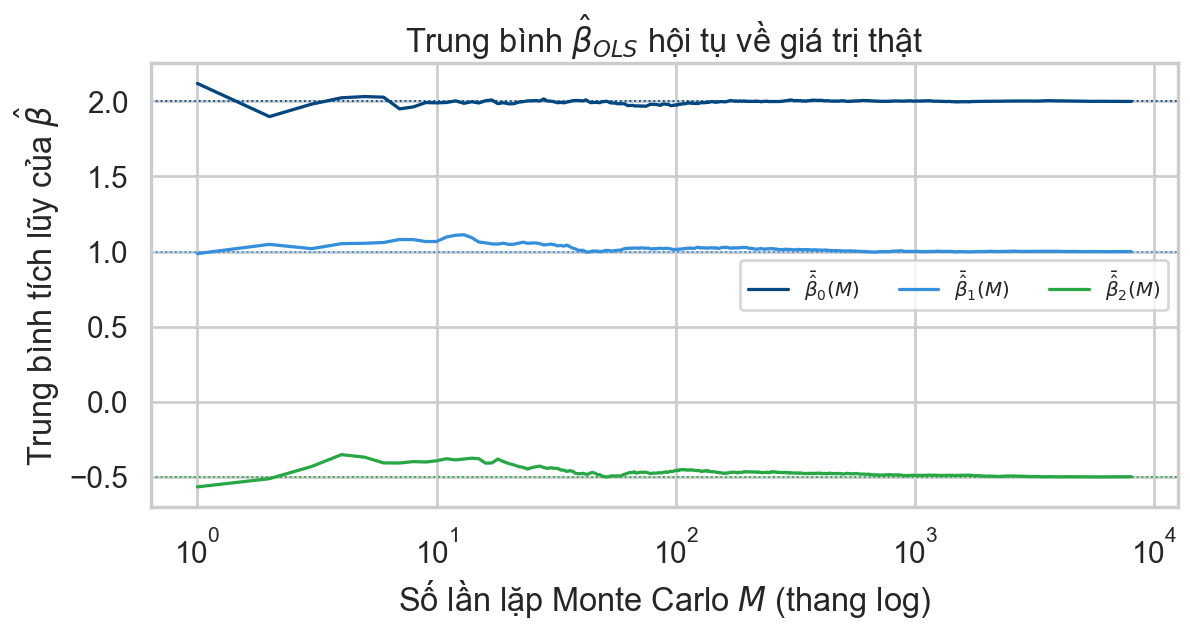
\includegraphics[width=0.82\textwidth]{images/fig_mc_convergence.png}
\caption{Trung bình tích lũy $\bar{\hat{\boldsymbol{\beta}}}(M)$ theo số lần lặp (thang log).
Cả ba thành phần hội tụ về giá trị thật $2.0,\ 1.0,\ -0.5$ (đường chấm).}
\label{fig:mc_conv}
\end{figure}

\noindent\textbf{Nhận xét.} Khi $M$ nhỏ, trung bình dao động mạnh do ít mẫu; khi $M$ tăng,
cả ba đường \textbf{ổn định và bám sát} đúng giá trị thật. Đây là biểu hiện của luật số lớn
cho $\E[\hat{\boldsymbol{\beta}}_{\mathrm{OLS}}] = \boldsymbol{\beta}$. Bảng~\ref{tab:mc_results}
cũng cho thấy độ chệch của \textit{cả} OLS lẫn Alt đều $\le 4.6\times10^{-3}$ --- nhỏ hơn
nhiều so với độ phân tán của ước lượng. (Độ chệch thực nghiệm của Alt hơi lớn hơn OLS chỉ
vì phương sai lớn hơn nên sai số Monte Carlo của trung bình cũng lớn hơn, không phải thiên
lệch hệ thống.)

\paragraph{(2) Phương sai nhỏ nhất.}
Hình~\ref{fig:mc_compare} chồng phân phối lấy mẫu của OLS (xanh) và Alt (cam) cho từng hệ số.
\textbf{Cách đọc:} mỗi ô là phân phối của một hệ số; vạch đỏ là giá trị thật.

\begin{figure}[H]
\centering
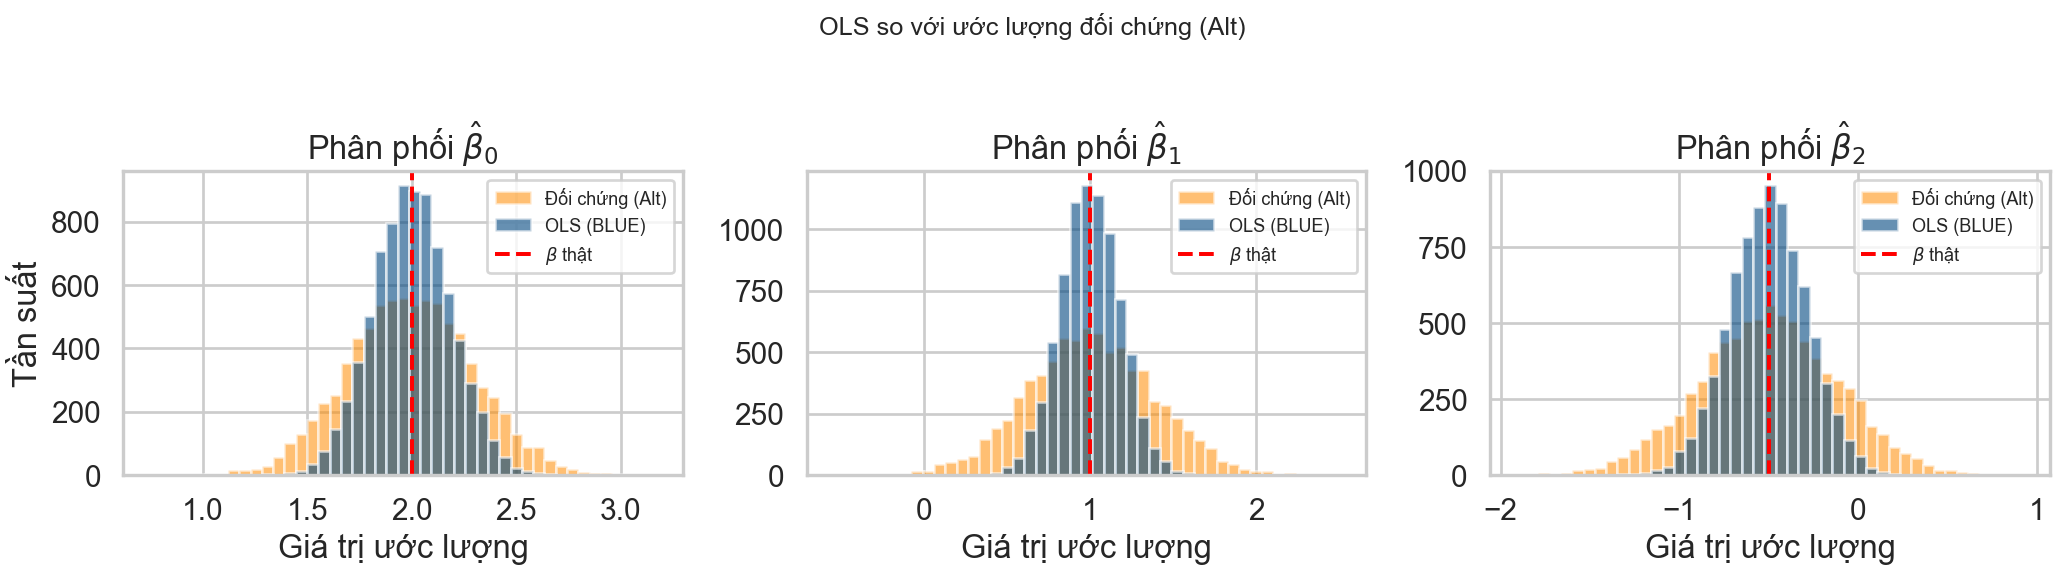
\includegraphics[width=\textwidth]{images/fig_mc_comparison.png}
\caption{Phân phối lấy mẫu OLS (xanh) vs Alt (cam) theo từng hệ số. Cả hai cùng tâm tại
$\boldsymbol{\beta}$ thật (vạch đỏ đứt), nhưng OLS hẹp hơn rõ rệt.}
\label{fig:mc_compare}
\end{figure}

\noindent\textbf{Nhận xét.} Cả hai phân phối đều \textbf{cùng tâm} tại giá trị thật (vạch đỏ)
--- OLS và Alt đều không chệch. Nhưng phân phối OLS (xanh) \textbf{cao và hẹp hơn}, tức tập
trung quanh $\boldsymbol{\beta}$ chặt hơn; Alt (cam) trải rộng hơn ở cả ba hệ số. Đây là minh
họa trực quan cho việc OLS có phương sai nhỏ nhất (BLUE).

Hình~\ref{fig:mc_var} lượng hóa điều đó theo \textit{từng} hệ số. \textbf{Cách đọc:} mỗi hệ
số có 4 cột --- OLS (Monte Carlo), OLS (lý thuyết), Alt (Monte Carlo), Alt (lý thuyết).

\begin{figure}[H]
\centering
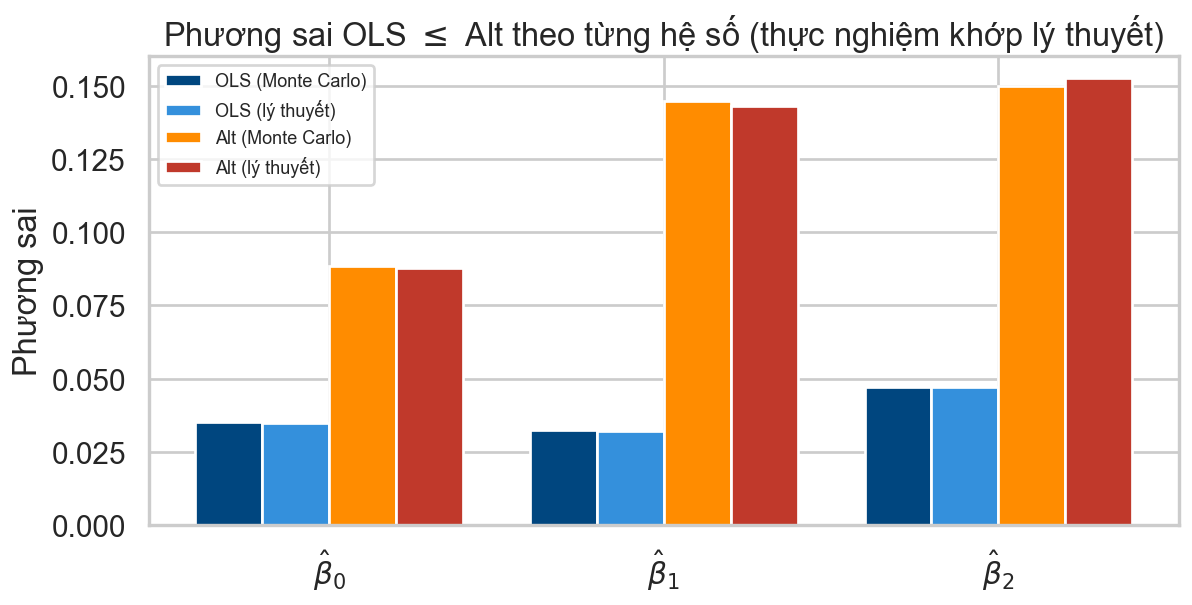
\includegraphics[width=0.82\textwidth]{images/fig_mc_variance.png}
\caption{Phương sai theo từng hệ số: với mỗi hệ số, cặp cột Monte Carlo và lý thuyết gần
như bằng nhau; cột Alt luôn cao hơn cột OLS.}
\label{fig:mc_var}
\end{figure}

\noindent\textbf{Nhận xét.} Với mỗi hệ số, cột \textbf{Monte Carlo} và cột \textbf{lý thuyết}
gần như bằng nhau --- mô phỏng khớp công thức $\sigma^2(\mat{X}^T\mat{X})^{-1}$
\eqref{eq:ols_cov} và $\mathrm{Var}(\hat{\boldsymbol{\beta}}_{\mathrm{OLS}}) + \sigma^2\mat{A}\mat{A}^T$
\eqref{eq:alt_var}. Cột Alt cao hơn cột OLS ở \textbf{mọi} hệ số (tỉ số $\approx 2.5$--$4.5$),
khẳng định OLS có phương sai nhỏ hơn --- đúng kết luận BLUE.

\subsubsection{Kiểm chứng với NumPy và scikit-learn}

Để bảo đảm cài đặt từ đầu là chính xác, ta so nghiệm OLS thu được trên một mẫu với hai
công cụ chuẩn: \texttt{numpy.linalg.lstsq} và
\texttt{sklearn.linear\_model.LinearRegression} (đặt \texttt{fit\_intercept=False} vì cột
hệ số tự do đã nằm trong $\mat{X}$).

Hàm \texttt{verify\_with\_numpy\_sklearn()} trong \texttt{code/monte\_carlo\_gauss\_markov.py}
thực hiện kiểm chứng này:

\noindent Kết quả kiểm chứng:
\begin{itemize}[noitemsep, leftmargin=1.4cm]
    \item $\norm{\hat{\boldsymbol{\beta}}_{\text{tự xây dựng}}
          - \hat{\boldsymbol{\beta}}_{\text{NumPy}}}_\infty
          = 6.66\times10^{-16}$ \quad (đạt độ chính xác máy).
    \item $\norm{\hat{\boldsymbol{\beta}}_{\text{tự xây dựng}}
          - \hat{\boldsymbol{\beta}}_{\text{sklearn}}}_\infty
          = 6.66\times10^{-16}$.
    \item Phương sai thực nghiệm Monte Carlo khớp công thức lý thuyết ở mọi hệ số
          (xem Bảng~\ref{tab:mc_results}).
\end{itemize}

\begin{note}[Kết luận]
Mô phỏng Monte Carlo xác nhận đầy đủ Định lý Gauss--Markov: ước lượng OLS \textbf{không
chệch} (trung bình trùng giá trị thật) và có \textbf{phương sai nhỏ nhất} so với ước lượng
tuyến tính không chệch đối chứng (Alt). Cài đặt từ đầu trùng khớp NumPy/scikit-learn tới
độ chính xác máy, và phương sai thực nghiệm khớp công thức $\sigma^2(\mat{X}^T\mat{X})^{-1}$.
\end{note}
